% CREATED BY DAVID FRISK, 2015
\chapter{Introduction}
\lettrine[findent=2pt]{\fbox{\textbf{T}}}{ }his Master's thesis report presents the results from identifying key components of the architectures for the electrical system in Volvo Car Group in order to create automated visualization of the architectures, which is derived from the needs of different stakeholders. This report also includes the results from an evaluation of how the automated visualizations affect the way of working with Electrical Power System (EPS) and in the electrical department of the company.

\section{Background}\label{Background_ref}
One of the biggest challenges in automotive industry during the past few years is to build vehicles that meet customer expectations. To overcome the challenge, more complex system of mechanical and electrical components is designed for and built in modern vehicles. Besides, software is also integrated in order to carry out some tasks, resulting in more than a hundred of Electrical Control Unit (ECU) deployed in a car. For this reason, creating architecture the complex system is of importance to ensure that every components and the communication among them are in the right places. \\

Volvo Car Group is a Swedish premium automotive manufacturer producing modern vehicles to the world. At the company, two types of architectures for electrical system are used to handle complex systems for cars \cite{Eliasson_1}. These two architectures are created with different abstract levels, meaning that they serve different purposes. A high-level architecture (logical view) containing Logical Architectural Components (LAC) is designed by software architects with its purpose is to guide and breakdown work to be developed during implementation phase. Development team creates a low-level architecture (design view) representing actual structure of an electrical system. It contains smaller Logical Components (LC) which are broken down from LACs in the high-level architecture, communication among LCs, and signals they receive/send. The low-level architecture is stored in a proprietary tool called \textit{Elektra} in which some related data such as mapping information between software components and ECUs, and deployment information are stored. With the data, the tool can generate model shells to be implemented by software developers for in-house software development, and requirement documents for functionality to be implemented by suppliers. Moreover, it can also generate ECU-integration and network communication in the electrical system \cite{Eliasson_2}.\\

\begin{figure}[H]
\centering
\captionsetup{justification=centering}
\vspace{0cm}% Adjust vertical spacing here

\includegraphics[width=0.4\linewidth]{figure/temp.png}
\caption{Low- and high-level architectures of an electrical system.}
\end{figure}

The low-level architecture that can be seen in the proprietary tool Elektra is a complete view of the whole electrical system. The tool does not allow users to select and generate visualization of some parts of the system. The architecture is enormous since it contains all LC and their communication, making them difficult for both teams and other stakeholders to see. \todo{[insert more text]}

\section{Statement of the problem} \label{Statement_ref}
The first problem that this thesis work addresses is, the current software Elektra shows the irrelevant parts of the architectural diagram. It shows the complete architecture including all components, ports, and their interactions among them. Moreover, the tool does not have visualization. In most cases, only some parts of the diagrams are relevant to the stakeholders which depends on each individual’s interest. This makes the architectural diagrams difficult for them to understand. Furthermore, the diagram at VCG does not only contain the components, ports, and connections, but also a logical designs. This makes the document even bigger and harder for stakeholders to focus on only the parts that they have an interest in. \\ 

The second problem is, the inconsistency between the low-level and high-level architectures. Usually, the stakeholders who interact with the system may have certain features that are required to be implemented in the system. When the developers implement these features in a system, they are also required to update the low-level architecture regularly. So, this is the point where the inconsistency occurs. 

To tackle these two problems, our thesis will provide a solution which helps to create automated visualization of the current status of Elektra with regard to the main interests of different stakeholders, also the solution will help high-level architects to get better understanding of what is going on in the real implementation which can support a decision making.


\section{Purpose} \label{Purpose_ref}
The purpose of this thesis work is to find metrics that helps to identify the key components of the electrical architectures and to understand their viewpoints on a visualization of the system. This thesis also aims to find and create possible views or visualizations of the electrical architectures with regards to the interests of different stakeholders, rather than the complete view from Elektra. The metrics found are used as inputs to a visualization tool in order to create the visualization of the key components of the electrical architectures.

\section{Research questions} \label{RQ_ref}
In order to achieve the goals, we address the following research questions:

\begin{que} \label{que:1}
What are the needs of stakeholders towards the visualization of the architectural diagrams?
\end{que}

\begin{que} \label{que:2}
What are the needs of stakeholders towards the visualization of the architectural diagrams?
\end{que}

\begin{que} \label{que:3}
What are the differences of the needs from each stakeholder?
\end{que}

\begin{que} \label{que:4}
How do we identify the needs of stakeholders and come up with software metrics that can help to identify important components in the architectural diagrams?
\end{que}

\begin{que}\label{que:5}
How do we complement Elektra with a visualization tool?
\end{que}

\begin{que} \label{que:6}
How does the automated visualization of the architectural diagrams impact the way of working?
\end{que}


\section{Limitation} \label{Limitation_ref}
The first procedure that was followed was to conduct interview sessions with different stakeholders at Volvo Car Group and to find out what the important components that they want to see in the electrical architectures were. However, there are some limitation to the work at the time of the study. Firstly, only a small group consisting of [---]\todo{insert number of stakeholders} stakeholders was selected to participate in identifying the key components due to time limitation which made it impossible to involve all stakeholders. \\

Secondly, the visualization tool that was used together with the metrics that were discovered from the stakeholders might be specific and perhaps the results of the visualization could not be the same if any other different tool was used. \\

Lastly, the visualization that was achieved using the metrics might not be applicable to other groups of stakeholders, or in other companies. The thesis work is performed at Volvo Car Group and hence the metrics that were discovered might only be applicable in the company or similar company where the same way of modelling electrical architectures is created.


\section{Outline of the report} \label{Outline_ref}
This report is divided into 6 chapters which can be seen in . 
\begin{figure}[H]
\centering
\captionsetup{justification=centering}
\vspace{0cm}% Adjust vertical spacing here
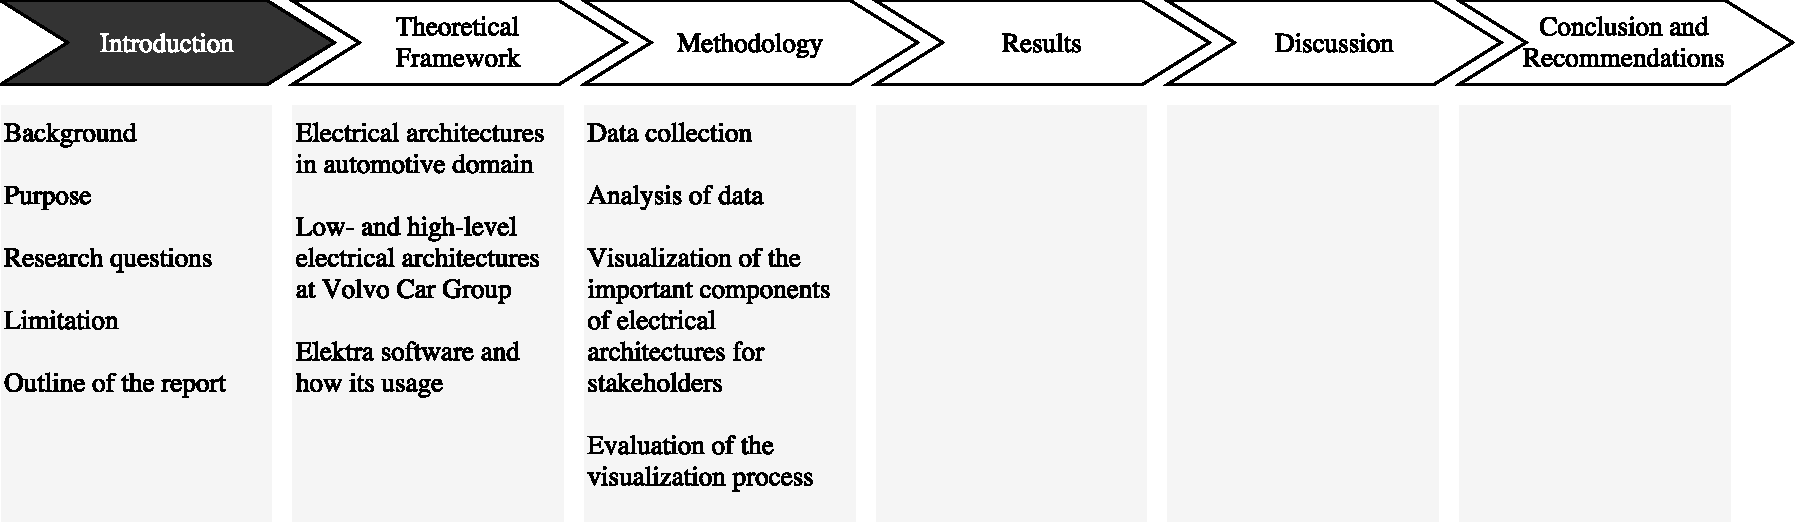
\includegraphics[width=1\linewidth]{figure/report_outline.pdf}
\caption{Report outline}
\end{figure}